\section{Auswertung}
\label{sec:Auswertung}
\subsection{Geschwindigkeit des Wagens}
Zur Bestimmung der Geschwindigkeiten für die zehn Gänge wird die Formel
\begin{align}
  v=\frac{s}{t}
\end{align}
genutzt. Für die Strecke gilt $s=(0,450\pm0,005)$m.
Die gemittelten Geschwindigkeiten finden sich in Tabelle \ref{tab:v} wieder.
\begin{table}
  \centering
  \caption{Geschwindigkeit des Wagens bei unterschiedlichen Gängen}
  \label{tab:v}
  \begin{tabular}{c c c}
    \toprule
    $Gang$ & $Geschwindigkeit\ \overline{\text{v}}/\si{\meter\per\second}$ & $\sigma_{\text{v}}$\\
    \midrule
    6  & 0,102 & 0,001\\
    12 & 0,204 & 0,002\\
    18 & 0,307 & 0,003\\
    24 & 0,410 & 0,005\\
    30 & 0,512 & 0,006\\
    36 & 0,616 & 0,007\\
    42 & 0,720 & 0,008\\
    48 & 0,821 & 0,009\\
    54 & 0,92  & 0,01\\
    60 & 1,03  & 0,01\\
    \bottomrule
   \end{tabular}
\end{table}\\
Nun soll untersucht werden, ob bei den hier verwendeteten Geschwindigkeiten
ein Unterschied zwischen Formel \eqref{eqn:frequenzempf}, für den bewegten Empfänger,
und der Formel \eqref{eqn:frequenzsender} für den bewegten Sender.
Dafür wird die höchste Geschwindigkeit, die in dem Versuch vorkommt,
hier die Geschwindigkeit des Ganges 60,in die Formeln eingesetzt
und beide Ergebnisse miteinander Verglichen:
\begin{align}
  \nu_E&=(20,80\pm0,02)\si{\second\tothe{-1}}\\
  \nu_Q&=(21,7444\pm0,0001).
\end{align}
Der Unterschied zwischen $\nu_E$ und $\nu_Q$ beträgt circa 1 kHz, und ist damit
vernachlässigbar. Somit lässt sich in diesem Versuch immer die Formel \eqref{eqn:frequenzempf}
verwenden.

\subsection{Wellenlänge }
Für die gemittelte Wellenlänge ergibt sich:
\begin{align}
  \overline{\lambda_0}=(17,5\pm 0,6) \si{\milli\meter}.
\end{align}
Mit dem Kehrwert:
\begin{align}
\frac{1}{\lambda_0}=(0,057\pm 0,002) \si{\per\meter}
\end{align}
ergibt sich aus der Beziehung $c=\nu_0\cdot\lambda_0$ für $\frac{\nu_0}{c}$
derselbe Wert.

\subsection{Frequenzmessung}
Wie in Kapitel \ref{sec:Frequenzmessung} beschrieben, werden die
Frequenzen abhängig von der Geschwindigkeit gemessen.
In den Tabellen \ref{tab:vorwärts} und \ref{tab:rückwärts} sind
die Mittelwerte der gemessenen Frequenzen
für die entsprechenden Geschwindigkeiten aufgetragen.
Die gemessene Ruhefrequenz $\nu_0$ beträgt:
\begin{align}
  \nu_0=20,74443\text{kHz}
\end{align}
Durch die zuvor gemessenen Wellenlänge $\lambda_0$
und der Ruhefrequenz $\nu_0$ lässt sich aus der Formel \eqref{eqn:c}
die Ausbreitungsgeschwindigkeit $c$ bestimmen:
\begin{align}
  c=(364,0\pm12,6)\si{\meter\per\second}
\end{align}
Da $v_{max}\ll c$ ist, führt dies ebenfalls zu der Abschätzung
$\nu_E \approx \nu_Q $.
\begin{table}
  \centering
  \caption{Gemittelte Frequenzenzen für die Bewegung auf das Mikrophon zu.}
  \label{tab:vorwärts}
  \begin{tabular}{c c c c c}
    \toprule
Gang &  $ \overline{\text{v}} / \si{\meter\per\second}$ & $\sigma_{\text{v}}$
 & $\overline{\nu}/\si{\kilo\hertz}$ & $\sigma_{\nu}$\\
    \midrule
    6  & 0,051  & 0,0006 & 20,745  & 0,0\\
    12 & 0,102  & 0,001  & 20,7482 & 0,0004\\
    18 & 0,154  & 0,002  & 20,751  & 0,0\\
    24 & 0,205  & 0,002  & 20,7532 & 0,0004\\
    30 & 0,256  & 0,003  & 20,7562 & 0,0004\\
    36 & 0,308  & 0,004  & 20,7604 & 0,0005\\
    42 & 0,360  & 0,004  & 20,763  & 0,0\\
    48 & 0,410  & 0,005  & 20,7664 & 0,0005\\
    54 & 0,461  & 0,005  & 20,7692 & 0,0004\\
    60 & 0,513  & 0,006  & 20,772  & 0,0\\
    \bottomrule
  \end{tabular}
\end{table}
\begin{table}
  \centering
  \caption{Gemittelte Frequenzenzen für die Bewegung von den Mikrophon weg.}
  \label{tab:rückwärts}
  \begin{tabular}{c c c c c}
    \toprule
Gang &  $\overline{\text{v}}/\si{\meter\per\second}$ & $\sigma_{\text{v}}$
 & $\overline{\nu}/\si{\kilo\hertz}$ & $\sigma_{\nu}$\\
    \midrule
    6  & -0,051 & 0,0006   & 20,739  & 0,0\\
    12 & -0,102 & 0,001    & 20,7362 & 0,0004\\
    18 & -0,154 & 0,002    & 20,733  & 0,0\\
    24 & -0,205 & 0,002    & 20,73   & 0,0\\
    30 & -0,256 & 0,003    & 20,7272 & 0,0004\\
    36 & -0,308 & 0,004    & 20,724  & 0,0\\
    42 & -0,360 & 0,004    & 20,721  & 0,0\\
    48 & -0,410 & 0,005    & 20,718  & 0,0\\
    54 & -0,461 & 0,005    & 20,715  & 0,0\\
    60 & -0,513 & 0,006    & 20,7122 & 0,0004\\

    \bottomrule
  \end{tabular}
\end{table}


\subsection{Schwebungsmethode}
Bei der Schwebungsmethode muss beachtet werden, dass die
Geschwindigkeiten der unterschiedlichen Gänge mal 2
genommen werden müssen, da sich die Schallquelle,
hier der Reflektor,
zum Empfänger mit einer Geschwindigkeit
von 2v bewegt. Die gemittelten Werte des gemessenen $\Delta\nu$
für die verschiedenen Geschwindigkeiten
sind in der Tabelle \ref{tab:schwebung} dargestellt.

\begin{table}
  \centering
  \caption{Gemittelte Frequenzenzen für die Bewegung von den Mikrophon weg.}
  \label{tab:schwebung}
  \begin{tabular}{c c c c c}
    \toprule
Gang &  $\overline{\text{v}}/\si{\meter\per\second}$ & $\sigma_{\text{v}}$
 & $\overline{\Delta\nu}/\si{\kilo\hertz}$ & $\sigma_{\Delta\nu}$\\
    \midrule
    6  & 0,102 & 0,001 & 0,006  &0,0\\
    12 & 0,204 & 0,002 & 0,012  &0,0\\
    18 & 0,307 & 0,003 & 0,018  &0,0\\
    24 & 0,410 & 0,005 & 0,0257 &0,0005\\
    30 & 0,512 & 0,006 & 0,031  &0,0\\
    36 & 0,616 & 0,007 & 0,0367 &0,0005\\
    42 & 0,720 & 0,008 & 0,042  &0,0005\\
    48 & 0,821 & 0,009 & 0,049  &0,0\\
    54 & 0,92  & 0,01  & 0,055  &0,0\\
    60 & 1,03  & 0,01  & 0,061  &0,0\\
    \bottomrule
  \end{tabular}
\end{table}
\subsection{Lineare Ausgleichsrechnung}
Werden nun die Ergebnisse aus den Tabellen \ref{tab:vorwärts} bis \ref{tab:schwebung}
in den Abbildung \ref{abb:freq} und \ref{abb:schw} in der Form $v$ nach $\Delta\nu$ aufgetragen.
$\Delta\nu$ errechnet sich bei den Ergebnissen aus Tabelle \ref{tab:vorwärts} und \ref{tab:rückwärts}
mit Hilfe der folgenden Formel:
\begin{align}
\Delta\nu=\nu_E-\nu_0
\end{align}
Aus den Messwerten lässt sich nun mit Hilfe der lineare Regression
die Proportionalitätsfaktoren zwischen $\Delta\nu$ und v bestimmen.
Desweiteren lässt sich durch die Wellenlängenmessung ebenfalls eine Gerade mit Hilfe der Formel \eqref{eqn:aenderungempf}
berechnen, die ebenfalls in Abbildung \ref{abb:freq} und \ref{abb:schw} zu sehen ist.
\begin{figure}
\centering
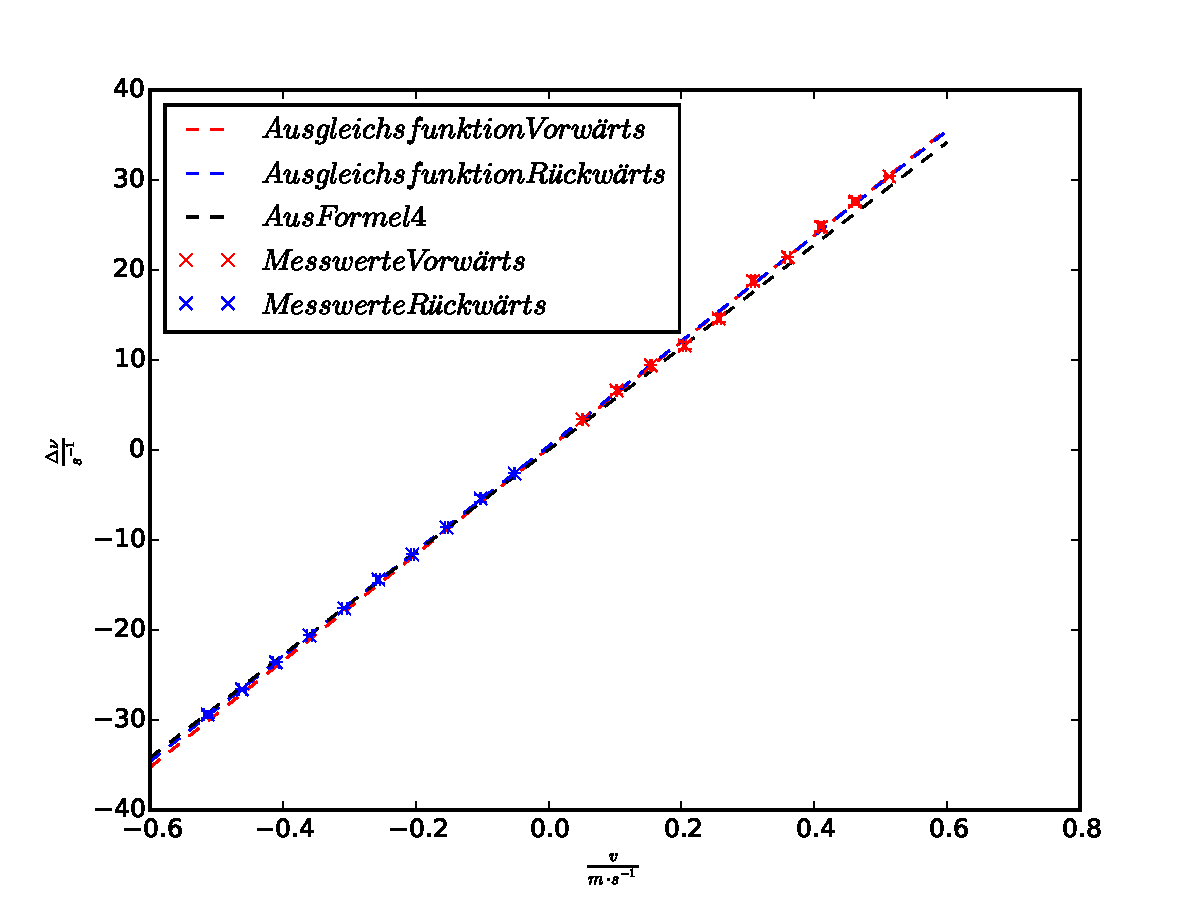
\includegraphics[width=0.7\textwidth]{graph.pdf}
\caption{Die Geschwindigkeit v nach $\Delta\nu $ aufgetragen für die Frequenzmessung $\nu$ durch den Aufbau aus der Abb:\ref{abb:Frequenzdiff}}
\label{abb:freq}
\end{figure}
\begin{figure}
\centering
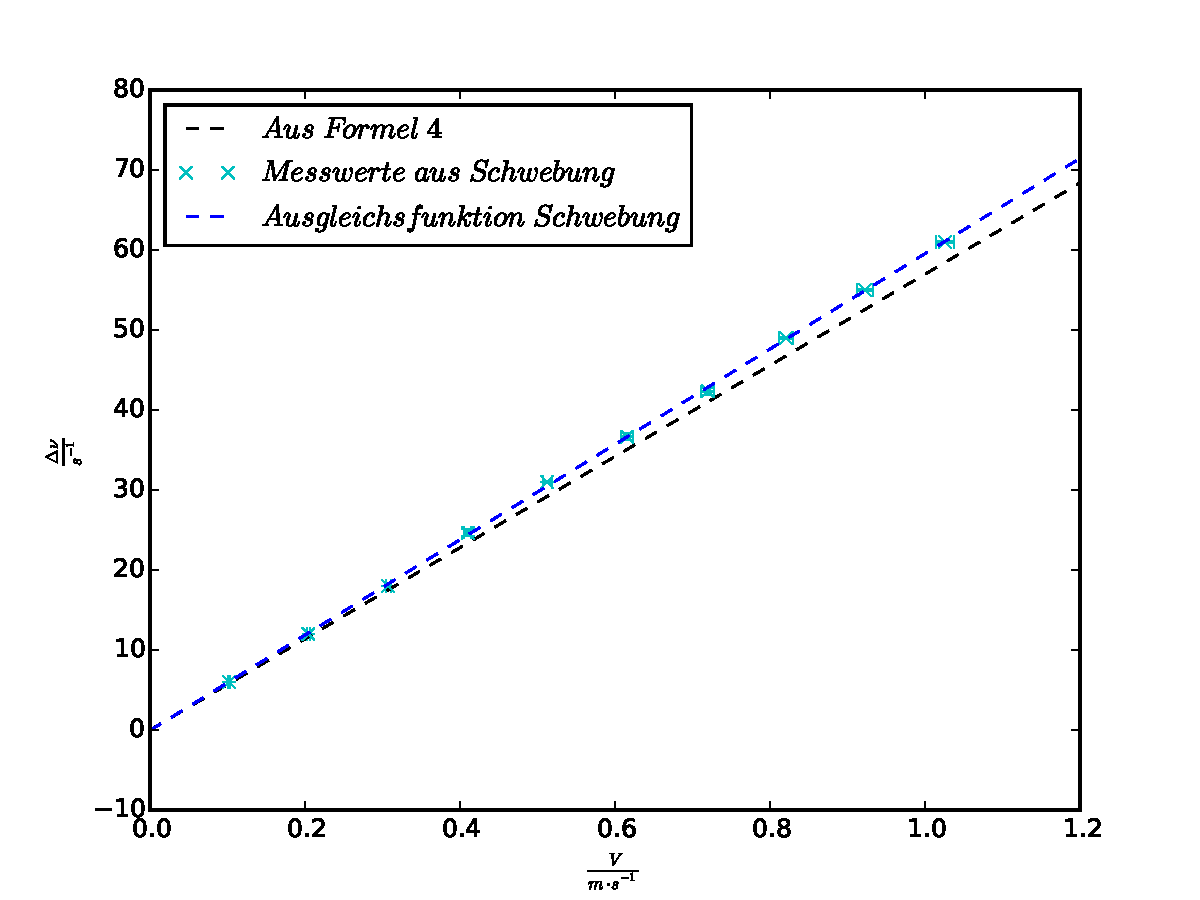
\includegraphics[width=0.7\textwidth]{graph2.pdf}
\caption{Die Geschwindigkeit v nach $\Delta\nu $ aufgetragen für die Messung von $\delta\nu$ durch den Aufbau aus der Abb:\ref{abb:Schwebung}}
\label{abb:schw}
\end{figure}
\FloatBarrier
Daraus ergibt sich der Proportionalitätsfaktor $\nu_0/c$ oder $1/\lambda$ für alle Messungen:
\begin{align}
   \text{Aus der Wellenlängenmessung:} \ &
   \frac{1}{\lambda} \ =(0,057\pm0,002)\si{\per\meter}\\
   \text{Aus der Frequenzmessung auf das Mikrophon zu:} \ &
   \frac{\nu_0}{c}=(0,059\pm0,001)\si{\per\meter}\\
\text{Aus der Frequenzmessung von dem Mikrophon weg:} \ &
\frac{\nu_0}{c}=(0,0584\pm0.0002)\si{\per\meter}\\
\text{Aus der Schwebungsmethode:} \ &
\frac{\nu_0}{c}=(0,0596\pm0,0003)\si{\per\meter}
\end{align}
